
\section{Non linearity and impact on CMB polarization measurements}
\label{sec:cmb}

Detecting CMB polarization $B$ modes is one of the major goals of modern
cosmology. However, due to the faintness of the expected signal, systematic
effects must be controlled to challenging low levels. In this context, the
knowledge of instrumental characteristics is one of many parameters that must be
well known. Linearity of the detector response is one of these,
and this section addresses its impact on measurements.

KIDs are presented in more details in Sect.~\ref{se:kids}. For now, we model
them as total power detectors placed right after a perfect polarizer whose
transmission direction makes an angle $\alpha$ w.r.t the sky local reference
axis (e.g. the longitude meridian). At each time, they therefore measure a
combination of the Stokes parameters $I$, $Q$ and $U$ of the total incident
radiation. If $\phi$ is the input power on the KID, to first order, the non
linearity of the KID response can be described by a parameter $\epsilon$ such
that the measure $m=\phi + \epsilon\phi^2$. Let us focus on the
extra contribution

\begin{eqnarray}
m &=& \phi + \epsilon\phi^2, \nonumber \\
&=& (I+Q\cos2\alpha+U\sin2\alpha) + \epsilon(I+Q\cos2\alpha+U\sin2\alpha)^2, \nonumber\\
 &\simeq & (I+Q\cos2\alpha+U\sin2\alpha) \nonumber \\
&+&\epsilon I^{2} + 2\epsilon IQ\cos2\alpha + 
2\epsilon IU \sin2\alpha + \mathcal{O}e^{i4\alpha}.
\label{eq:eq-NL}
\end{eqnarray}

In the following, we assume that the map making is able to discard the terms in
$4\alpha$ and to project only the spin-2 quantities. Non linearity couples total
intensity to polarization and creates spurious additional contributions to $Q$
and $U$, so that their estimates read

\begin{eqnarray}
\hat{I} &=& I + \epsilon I^2\\
\hat{Q} &=& Q + 2\epsilon IQ\\
\hat{U} &=& U + 2\epsilon IU
\end{eqnarray}

In addition to CMB, we must account for the foregrounds. We limit
ourselves to dust thermal emission and synchrotron because they are the two
major polarized foregrounds. The question is now to know how to include these
emissions, or their residuals after component separation, in our simulations to
assess the impact of non linearity on the final CMB estimates ? A complete study
of component separation is beyond the scope of this paper. However, for the sake of
specification derivation, it is enough to approximate foreground emissions by
fixed spatial templates at a reference frequency $\nu_0$ and power law
SED's. Let us denote $\beta_S$ and $\beta_D$ the indices of these power laws for
synchrotron and dust respectively. Thus

\begin{eqnarray}
I&=&I_{cmb} + \left(\frac{\nu}{\nu_0}\right)^{\beta_D}I_D(\nu_0) +
\left(\frac{\nu}{\nu_0}\right)^{\beta_S}I_S(\nu_0), \\
Q&=&Q_{cmb} + \left(\frac{\nu}{\nu_0}\right)^{\beta_D}Q_D(\nu_0) +
\left(\frac{\nu}{\nu_0}\right)^{\beta_S}Q_S(\nu_0), \\
U&=&U_{cmb} + \left(\frac{\nu}{\nu_0}\right)^{\beta_D}U_D(\nu_0) +
\left(\frac{\nu}{\nu_0}\right)^{\beta_S}U_S(\nu_0).
\end{eqnarray}

Putting these in eq.~(\ref{eq:eq-NL}), leads to:

\begin{eqnarray}
\hat{Q} &=& Q_{cmb} + 2\epsilon I_{cmb}Q_{cmb} \nonumber\\
&+&
2\epsilon\left(\frac{\nu}{\nu_0}\right)^{\beta_D}\left(I_{cmb}Q_D(\nu_0)+I_D(\nu_0)Q_{cmb}\right)\nonumber\\
&+&2\epsilon\left(\frac{\nu}{\nu_0}\right)^{\beta_S}\left(I_{cmb}Q_S(\nu_0)+I_S(\nu_0)Q_{cmb}\right) \nonumber\\
&+&2\epsilon\left(\frac{\nu}{\nu_0}\right)^{2\beta_D}I_D(\nu_0)Q_D(\nu_0) +
2\epsilon\left(\frac{\nu}{\nu_0}\right)^{2\beta_S}I_S(\nu_0)Q_S(\nu_0)\nonumber\\
&+&2\epsilon\left(\frac{\nu}{\nu_0}\right)^{\beta_D+\beta_S}\left(Q_D(\nu_0)I_S(\nu_0)+I_D(\nu_0)Q_S(\nu_0)\right),
\end{eqnarray}

with similar results for $\hat{I}$ and $\hat{U}$. Spectral dependence is the key
feature of component separation methods, and we assume in this work that it is
actually able to isolate components of a given SED, in particular that of the
CMB. This leads to the interesting result that all the couplings between
components have a SED that is different from that of the CMB. CMB will ``leak''
into components of the same SED as the foregrounds and foregrounds will induce
spurious components with SED's in $2\beta_D$, $2\beta_S$ and
$\beta_S+\beta_D$. So after component separation, we are left with

\begin{eqnarray}
\hat{I} &=& I_{cmb} +  \epsilon I_{cmb}^2, \label{eq:spurious-mapI}\\
\hat{Q} &=& Q_{cmb} + 2\epsilon I_{cmb}Q_{cmb}, \label{eq:spurious-mapQ}\\
\hat{U} &=& U_{cmb} + 2\epsilon I_{cmb}U_{cmb} \label{eq:spurious-mapU}.
\end{eqnarray}

We therefore build maps $\Delta I = I_{cmb}^2$, $\Delta Q = 2I_{cmb}Q_{cmb}$ and
$\Delta U = 2I_{cmb}Q_{cmb}$ and compute their angular power spectra
(Fig.~\ref{fig:power_spectra}). Requesting that the impact of non linearity be
lower than the cosmic variance on $C^{BB}_\ell$ at the $\ell=90$ peak leads to
$\epsilon \leq 2.6\times 10^{-5}$. In the next section, we show that KIDs are expected
to meet these requirements.

\begin{figure}
\center
\includegraphics[clip,angle=0,width=\columnwidth]{Figures/cmb_power_spectra.eps}
\caption{Power spectra for spurious temperature and polarization anisotropies of
  eq.~(\ref{eq:spurious-mapI}-\ref{eq:spurious-mapU}). These extra terms scale
  like $\epsilon$ at the map level, hence like $\epsilon^2$ on the $C_\ell$.}
\label{fig:power_spectra}
\end{figure}
